% !TeX document-id = {723fde2e-8374-4acb-a15d-4655fdd0b330}
% !TeX TXS-program:compile = txs:///pdflatex/[--shell-escape]
\pdfminorversion=7
%\RequirePackage[l2tabu, orthodox]{nag}
\documentclass[12pt,a4paper,twoside]{report}%report
%\usepackage[style=numeric, backend=bibtex]{biblatex}
\usepackage[style=numeric, backend=bibtex]{biblatex}
\addbibresource{cap/references.bib}
\usepackage{graphicx}
\usepackage[font=small,labelfont=bf]{caption}
\usepackage{hyperref}
\usepackage{subcaption}
%%%%%%
\usepackage[a4paper,width=150mm,top=25mm,bottom=25mm,bindingoffset=6mm]{geometry}
\usepackage[utf8]{inputenc}

%%fonts
%\usepackage{lmodern}
%\usepackage[qtm]{tgtermes}

\usepackage{xcolor}

%% code part
\usepackage{listings}
\usepackage{minted}
\usemintedstyle{bw}

%% TOREMOVE
\usepackage{easyReview}

%% ~
\usepackage{textcomp}
\newcommand{\mytexttilde}{\raisebox{0.5ex}{\texttildelow}}
%% error copy _
\usepackage[T1]{fontenc}
%\usepackage{lmodern}


%% pdf-A
%\usepackage[a-1b,mathxmp]{pdfx}[2018/12/22]
%\usepackage{colorprofiles}
%\usepackage{pdfa}

%\begin{filecontents*}[overwrite]{\jobname.xmpdata}
%	\Title{An implementation of Open-RMF in an industrial environment}
%	\Author{Michele Belletti}
%	\Language{en-GB}
%	\Subject{The abstract or short description.}
%	\Keywords{keyword1\sep keyword2\sep keyword3}
%\end{filecontents*}

\title{An implementation of Open-RMF in an industrial environment}
\author{Michele Belletti}
%\date{2025\\ December}

%\usepackage{blindtext}
%\usepackage{emptypage}
%\usepackage{graphicx}
%\usepackage{float}
%\usepackage{amsmath}
%\usepackage{gensymb}
%\usepackage{textcomp}
%\usepackage{booktabs}

%\usepackage{setspace}
%\setstretch{1.5}

%\usepackage{subcaption}

%\usepackage{multirow}

%\usepackage{natbib}
% modification to natbib citations
%\bibliographystyle{tmlr}
%\setcitestyle{authoryear,round,citesep={;},aysep={,},yysep={;}}

%\usepackage[format=hang,font=small,labelfont=bf]{caption}

%\usepackage{etoolbox}
%\renewcommand{\topfraction}{0.9}	% max fraction of floats at top
%\renewcommand{\bottomfraction}{0.8}	% max fraction of floats at bottom

%\setcounter{topnumber}{2}
%\setcounter{bottomnumber}{2}
%\setcounter{totalnumber}{4}     % 2 may work better
%\setcounter{dbltopnumber}{2}    % for 2-column pages
%\renewcommand{\dbltopfraction}{0.9}	% fit big float above 2-col. text
%\renewcommand{\textfraction}{0.07}	% allow minimal text w. figs

\begin{document}


\maketitle
\tableofcontents

\part{Introduction}
This work is a thesis on a new system OPEN-RMF still in development applied for a robot in the facility Elettra Sincotrone Trieste
\chapter{Background and motivation}
Elettra Sincontrone Trieste\footnote{https://www.elettra.eu/
} is a big research facility that, principally, gives to users two light sources: the synchrotron Elettra and the laser at free electron Fermi.
Besides this, it study new technology and technique to improve the capabilities and work activities. A lot of the latest improvements are based on robots, that also after the covid and latest with the exploding diffusion of LLMs, allow an interaction of the users of the light sources to communicates and interact with the robots in the facility to obtain information and services as transport of packages.
\chapter{Research questions and objectives}
\chapter{Scope and limitations}

\part{Literature Review}
In this part we will provide a description of the technologies used in this thesis. We will start describing what is ROS and how it works then we will talk about the navigation system used and how it is implemented the control with the fleet management system Open-RMF
\chapter{Overview of ROS1 and ROS2}
The Robotics Operating System \footnote{\href{https://www.ros.org/}{https://www.ros.org/}} is a compilation of tools and libraries open-source that help the development of application in the robotic environment. otherwise from the name, it's not a Operating System (OS) but an Software Development Kit (SDK) that gives at the user all the tools for creating your robot giving some typically functionality of an OS: hardware abstraction, low-level device control, implementation of commonly-used functionality, message-passing between processes, and package management.
The ROS ecosystem is based on (all these things is going to be described in detail in the next section):
\begin{itemize}
	\item An communication system named middleware or plumbing based on DDS (Data Distribution Service). This allow the Nodes to share information between each other with an anonymous publish/subscribe pattern allowing fault isolation, separation of concerns and clear interfaces and a synchronous system (remote procedure call)RPC-style communication between services.
	\item Tools to control and improve the development of the software like launch,  introspection, debugging, visualization, plotting, logging, and playback.
	\item Provides tools and libraries for obtaining, building, writing, and running code across multiple computers.
	\item A active and big community with at the center the Open Robotics\footnote{\href{https://www.openrobotics.org/}{https://www.openrobotics.org/}}.
\end{itemize}
\section{Structure of ROS}
The documentation\footnote{\href{https://docs.ros.org/en/rolling/index.html}{https://docs.ros.org/en/rolling/index.html}} give all the information of ROS, some functionality write below are not available for ROS 1:
\begin{itemize}
	\item The \textbf{ROS Graph} is a peer-to-peer network of processes that elaborated simultaneously and communicate with each other.
	\item \textbf{Nodes} is a modular process and should be a specific resolution for a problem to be more easily communicate with other Nodes through topics, services, action and parameters. They also can be based on LifecycleNode\label{LifecycleNode} that contain a state machine transitions for bringup and teardown to allow more deterministic behavior.
	\begin{figure}[h]
	\centering
	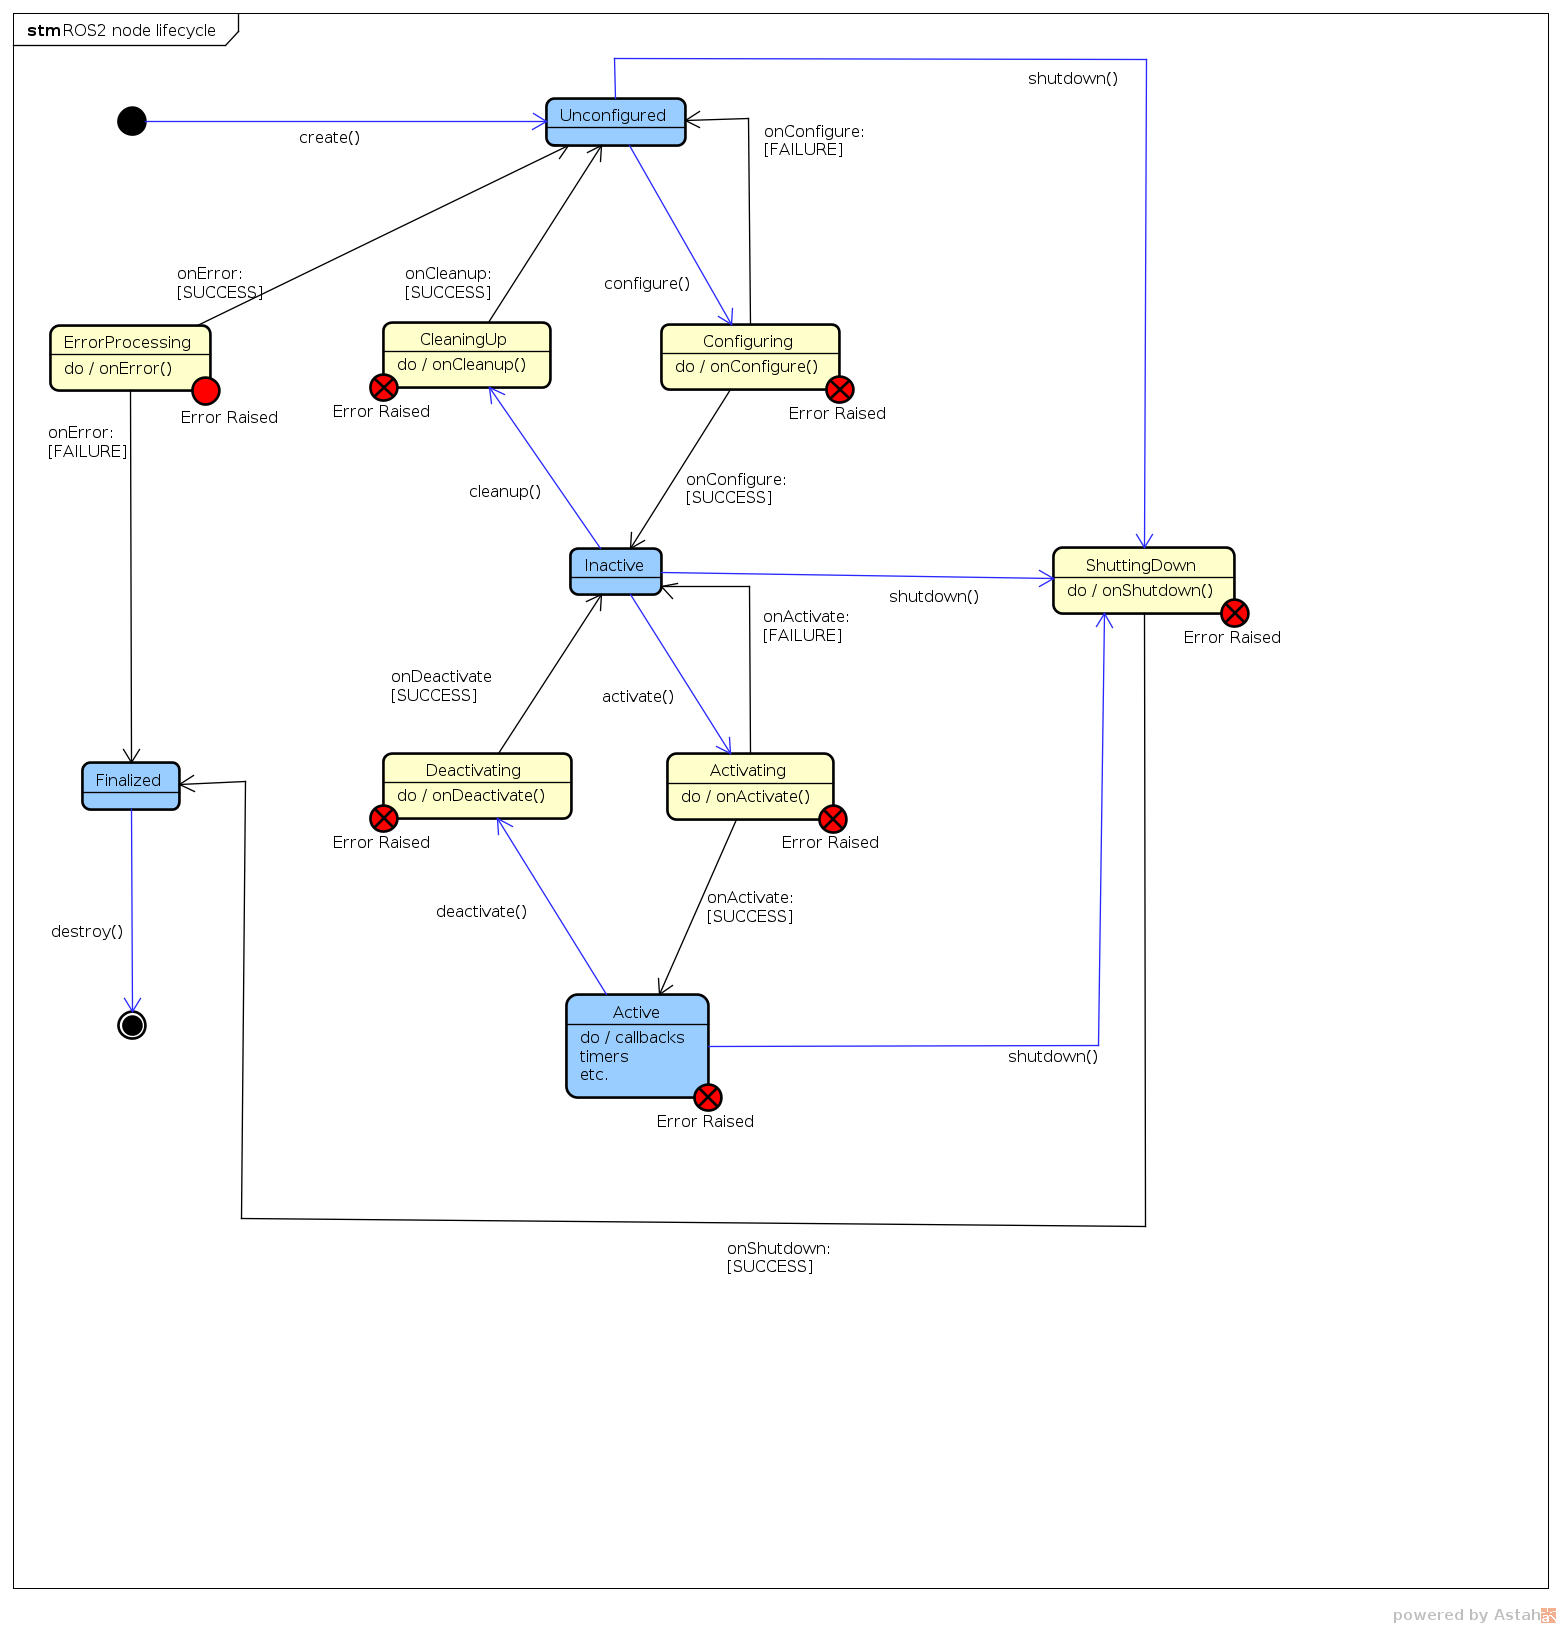
\includegraphics[width=0.8\linewidth]{img/life_cycle_sm.png}
	\captionof{figure}{State Machine of LifecycleNode}
	\end{figure}
	\item \textbf{Topics} are the bus for communication between Nodes to share a streams of messages in a publisher to subscriber structure.
	\begin{center}
		\captionsetup{type=figure}
		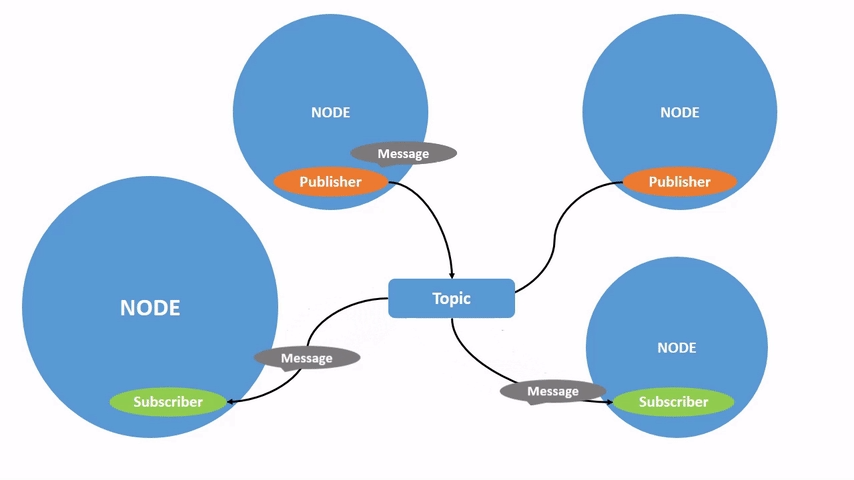
\includegraphics[width=0.49\linewidth]{img/Topic.png}
		\captionof{figure}{Topic process}
	\end{center}
	\item \textbf{Service} are based on the request and response model. When a node with a Service client send a Request Message to Node with a Service Server it will send a Response Message to that specific Service Client. 
	\begin{center}
		\captionsetup{type=figure}
		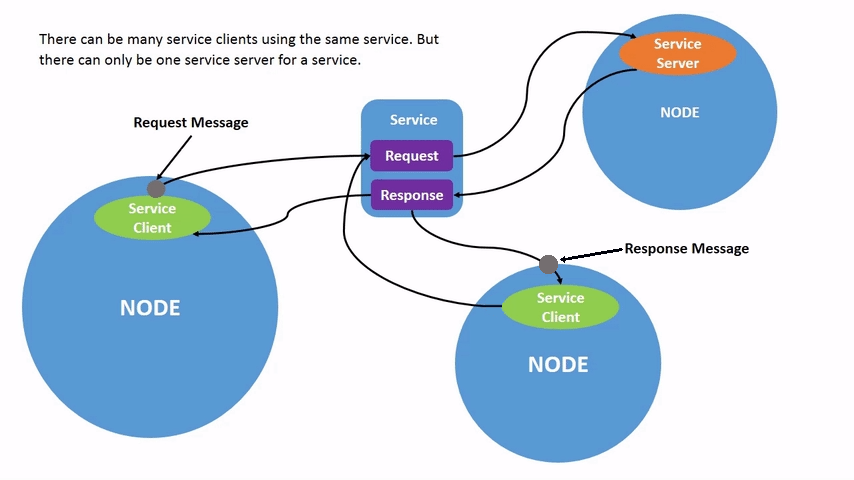
\includegraphics[width=0.49\linewidth]{img/Service.png}
		\captionof{figure}{Service process}
	\end{center}
	\item \textbf{Parameters} are configuration of a node and allow to modified them without changing the code.
	\item \textbf{Actions}\label{Action} were created to fulfill the needs of something for tracking long task. They are a combination of two service (goal and result) and a pub-sub (feedback). It send a goal request and receive a response then send a result request, the node then start to pub to the feedback topic and then response to the result request.
	\begin{center}
		\captionsetup{type=figure}
		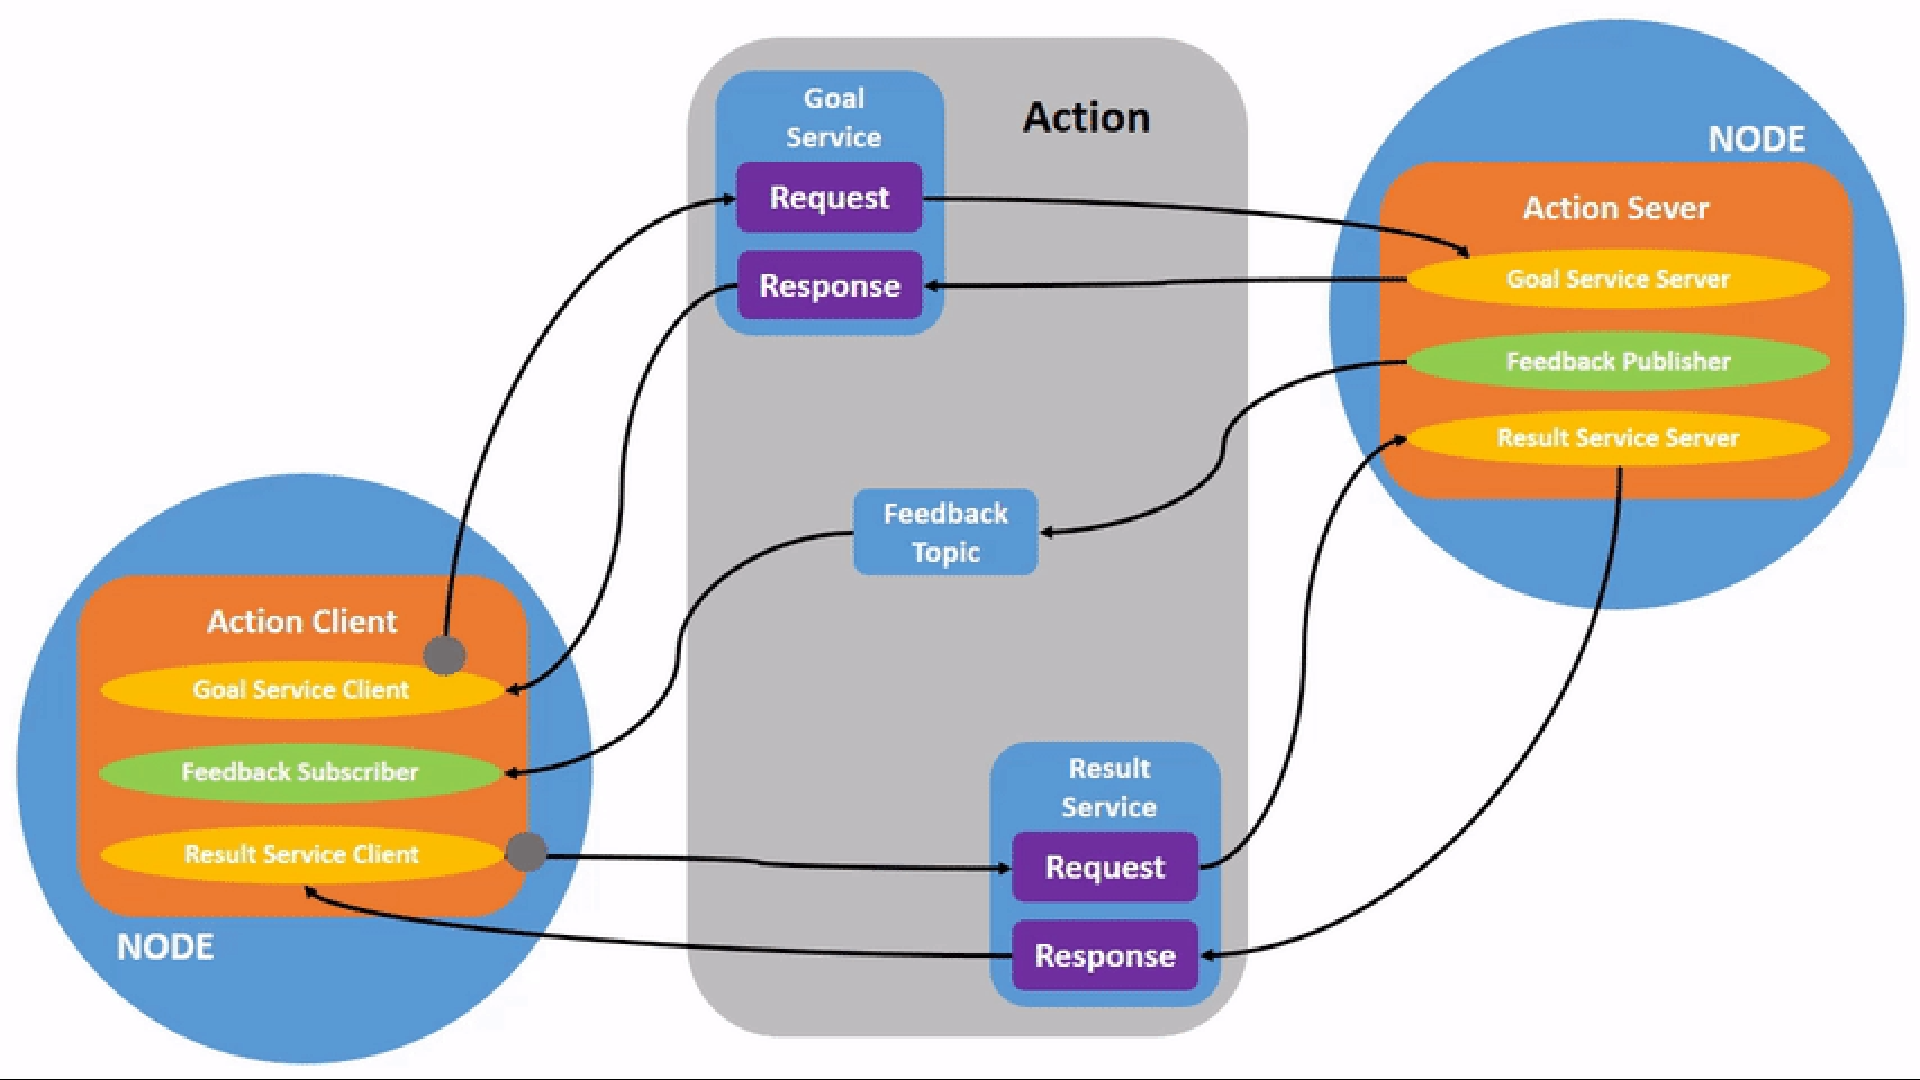
\includegraphics[width=0.49\linewidth]{img/Action.png}
		\captionof{figure}{Action process}
	\end{center}
\end{itemize}
\section{Tools of ROS}
Now i will describe the tools that are built in ROS for developing robotics system:
\begin{itemize}
	\item \textbf{Launch} is a file structure that allow to start multiple nodes with a set of parameters.
	\item \textbf{rqt} is a graphical user interface (GUI) tool for ROS 2. With a series of plugins allow to interact with an interface for helping in the development, in the monitoring and diagnostic the ROS system.
	\item \textbf{rqt\_console} visualize the log generate by the ROS 2 system.
	\item \textbf{Rviz} is a 3D visualizer for the Robot Operating System \underline{framework?}.
	\begin{figure}[h]
		\centering
		\begin{subfigure}{0.4\textwidth}
		\centering
		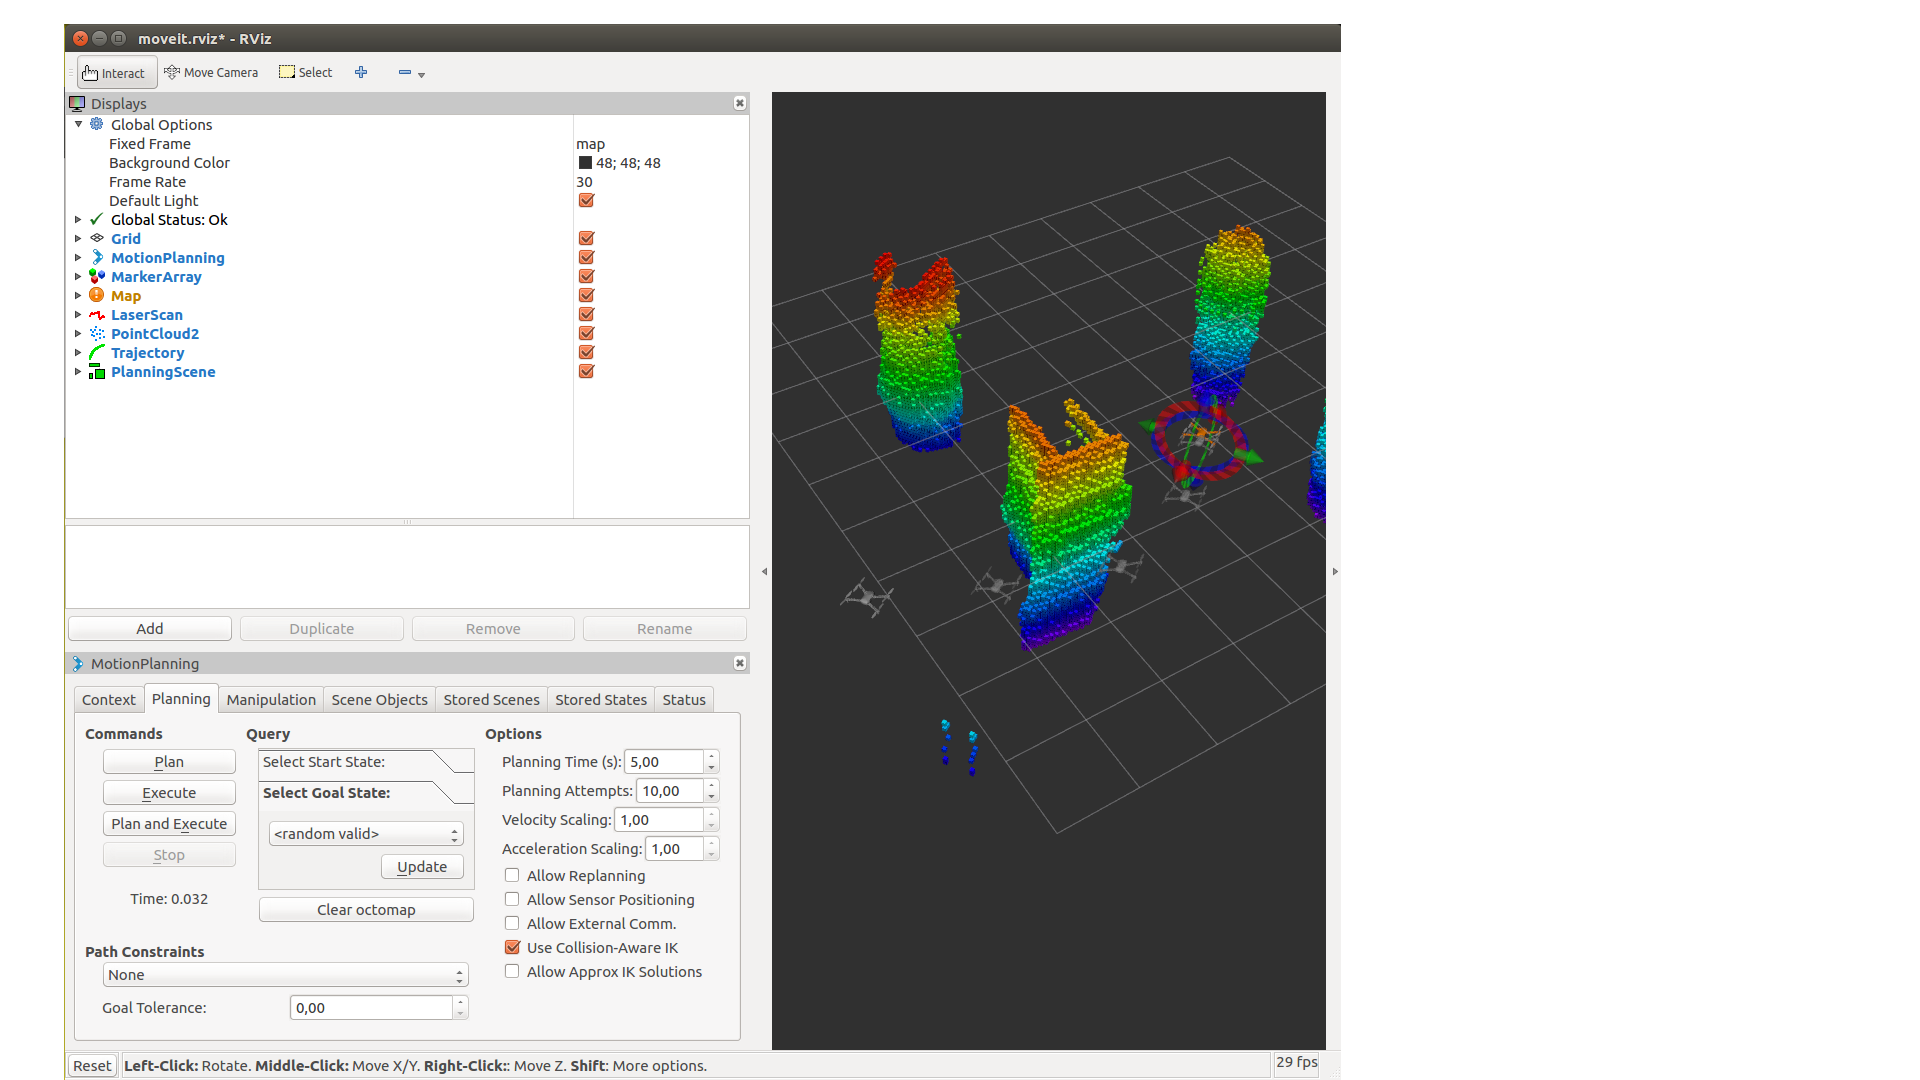
\includegraphics[width=0.9\linewidth]{img/rviz.png}
		\end{subfigure}
		\begin{subfigure}{0.4\textwidth}
		\centering
		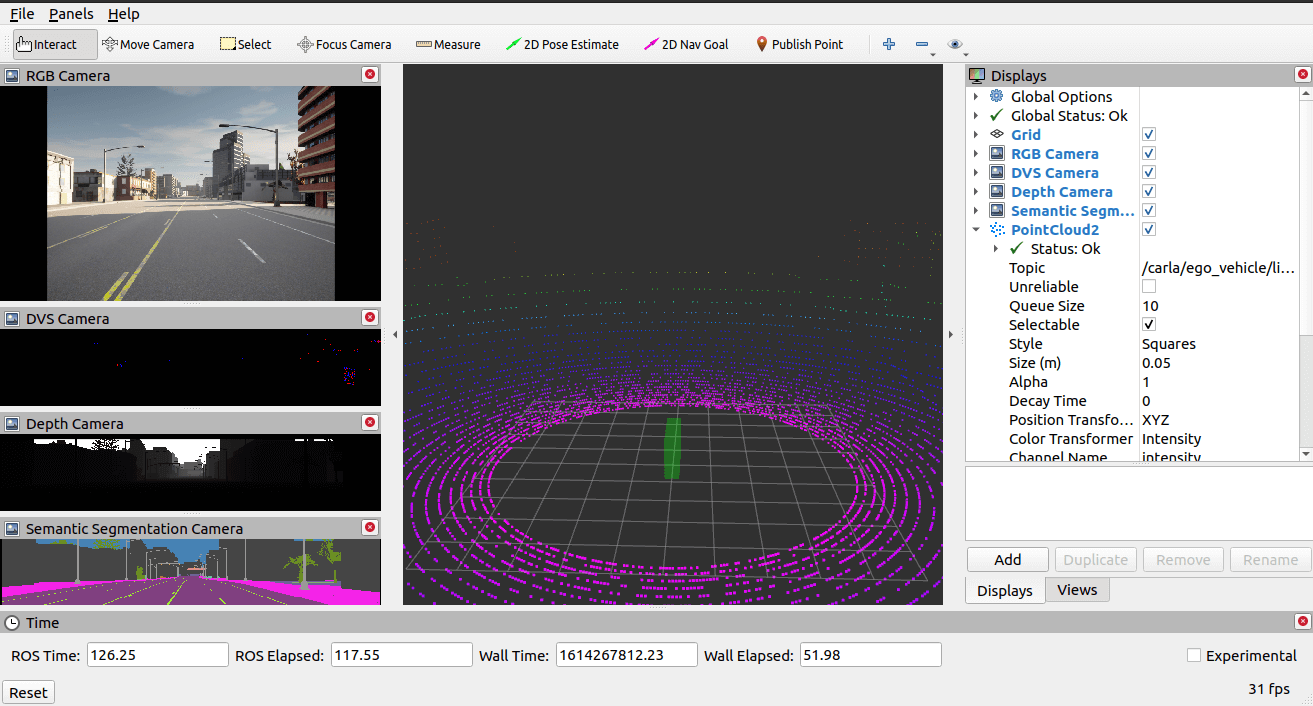
\includegraphics[width=0.9\linewidth]{img/rviz2.png}
		\end{subfigure}
		\captionof{figure}{Examples of visualization of ROS data with Rviz}
	\end{figure}
	\item \textbf{rosdep} is a dependency installer utility.
	\item \textbf{sros2} is a package that provide the tools and instruction to apply security on DDS.
\end{itemize}
Another tools that are connected with ROS and helps develop is the simulation environments. They allow to test the code on a simulated robot in different condition to find possible bugs in the code that if there was launched on a real robot can be harmful to it or the environment. They provide realistic physical mechanics at all the parts of simulation and in the documentation of ROS there are listened 2: Gazebo and Webots.
The first one is also a project under the Open Robotics and for a lot of projects is the default used like the one we will use.
Gazebo offer:
\begin{itemize}
	\item \textbf{ROS Integration} a bridge to converts the protobuf messages to ROS.
	\item \textbf{Performance tools} that allow to have it distributed on servers, dynamically asset loading and control of the time step for simulation to have the best performances.
	\item \textbf{Realistic simulation} that allow to insert a variety of sensor with their noise in a 3D rendering word built on Ogre 2.1\footnote{\href{https://wiki.ogre3d.org/Home}{https://wiki.ogre3d.org/Home}} and with the physic engine DART\footnote{\href{https://dartsim.github.io/}{https://dartsim.github.io/}}.
	\item \textbf{Extensibility} because its built on modularity, it allow with plugins to run code that interact with the simulation.	
\end{itemize}
	\begin{figure}[h]
		\centering
		\begin{subfigure}{0.4\textwidth}
			\centering
			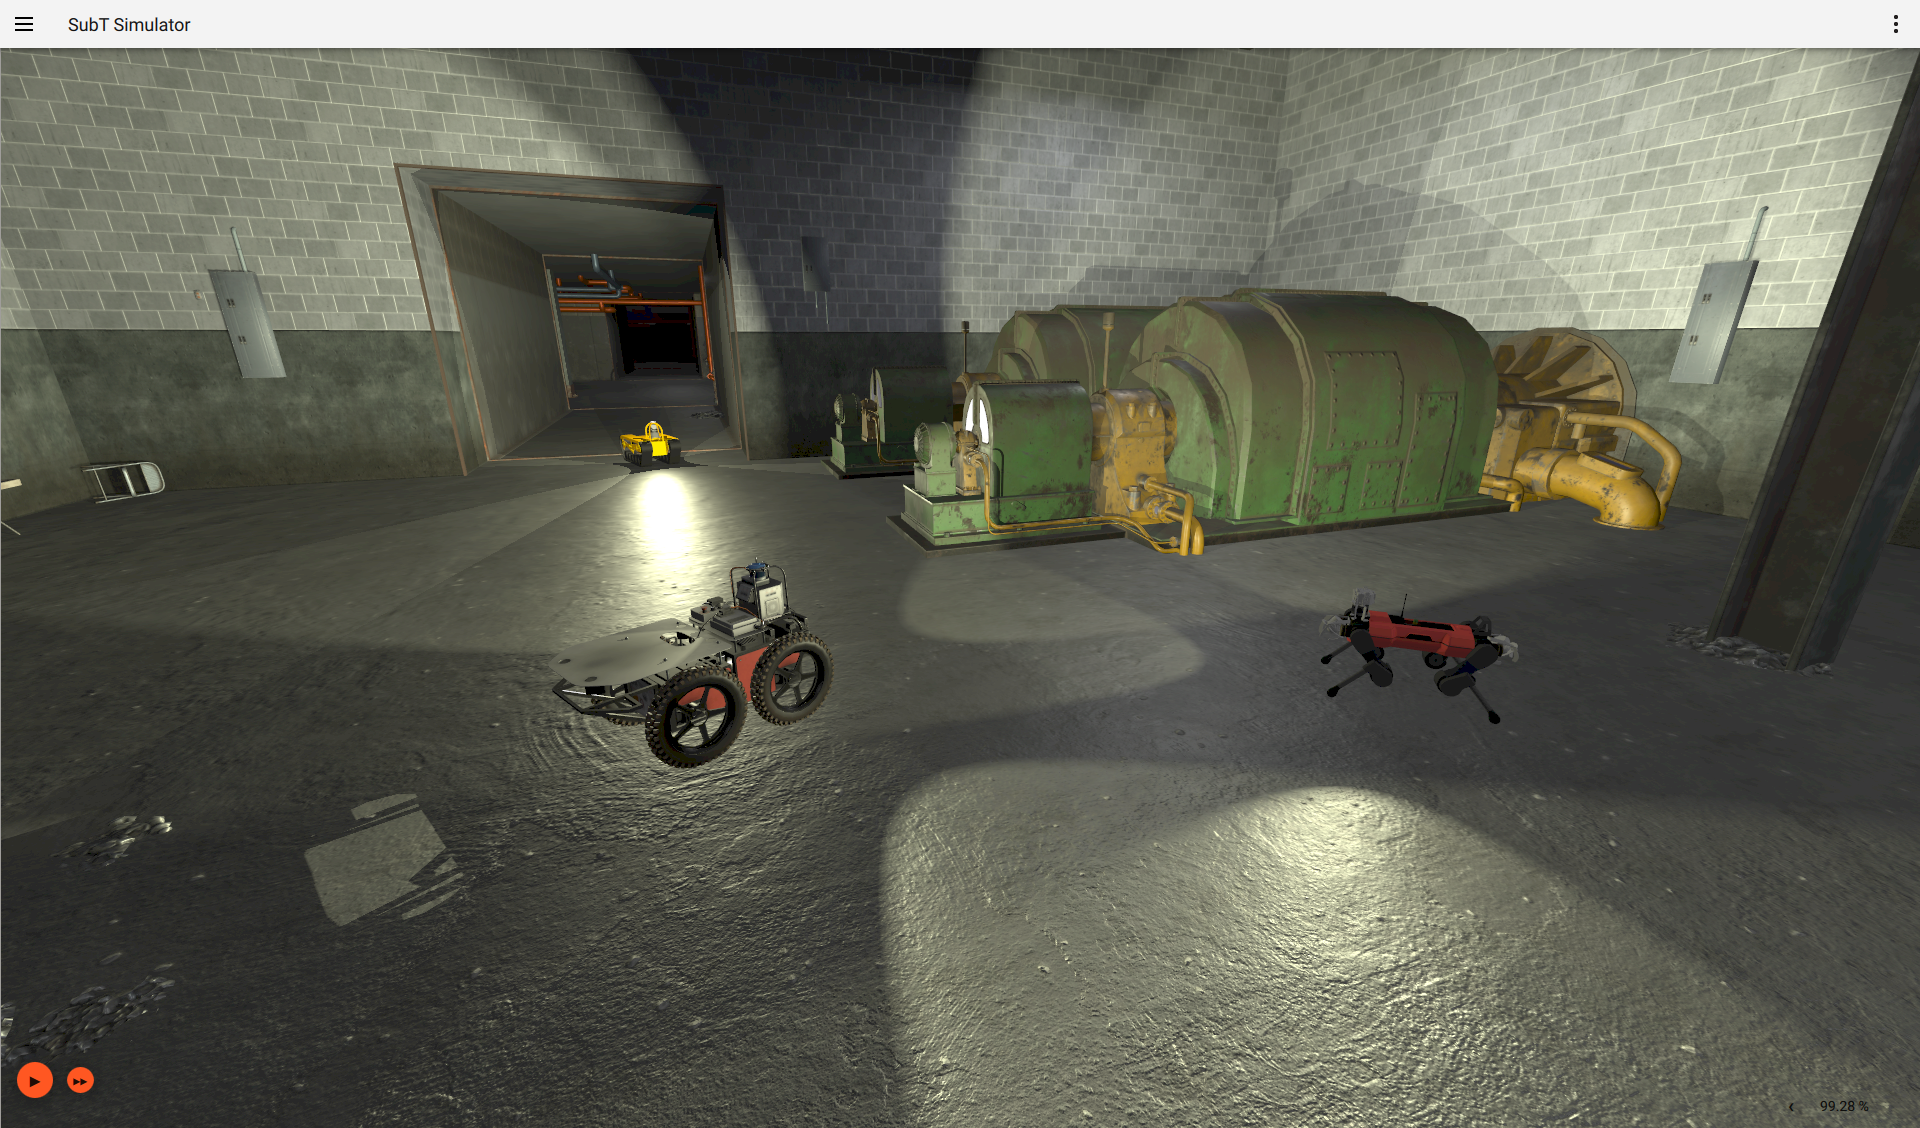
\includegraphics[width=0.9\linewidth]{img/gazebo1.png}
		\end{subfigure}
		\begin{subfigure}{0.4\textwidth}
			\centering
			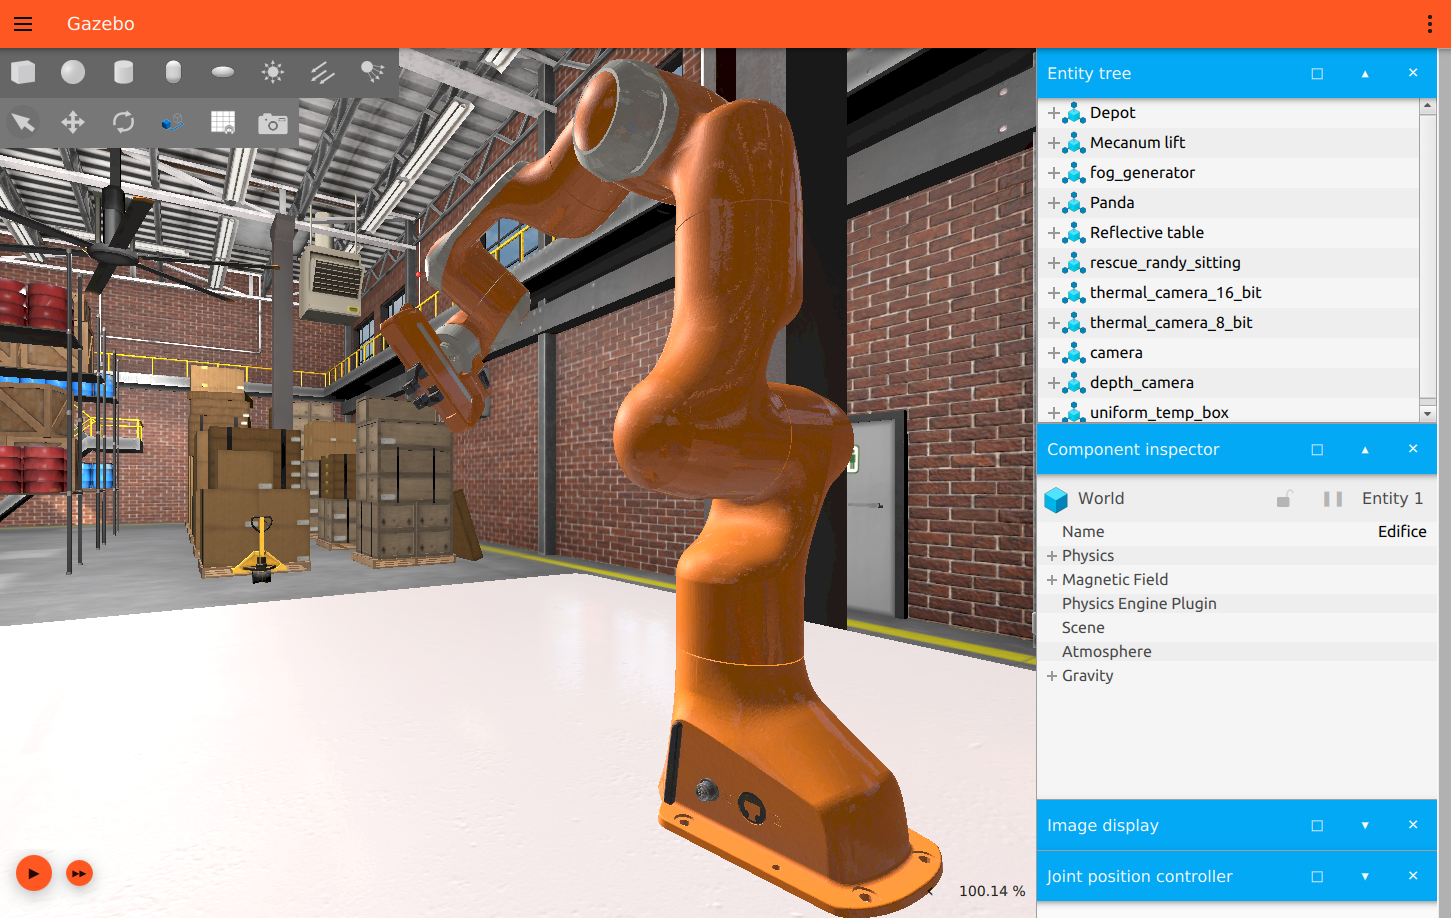
\includegraphics[width=0.9\linewidth]{img/gazebo2.png}
		\end{subfigure}
		\captionof{figure}{Examples of Gazebo}
\end{figure}
\chapter{Introduction to NAV2 and Google Cartographer}
Multiple tools are available for move a robot in an environment. The one that give a full system is Nav2
\footnote{\href{https://docs.nav2.org/}{https://docs.nav2.org/}}
\cite{macenski2020marathon2}
 the successor of ROS Navigation Stack of ROS 1.
\section{Description of Nav2}
Nav2 gives all the tools (perception, planning\cite{macenski2023survey}, control, localization, visualization) for whichever robot to navigate autonomously and reliably also thought hard environment. It allow to build a model of the environment from the data of the sensors, calculated dynamically the best path to follow to avoiding obstacles using a map, set the velocity of the motors and allow to follow logic step using a behaviors tree.
\begin{figure}[h]
\centering
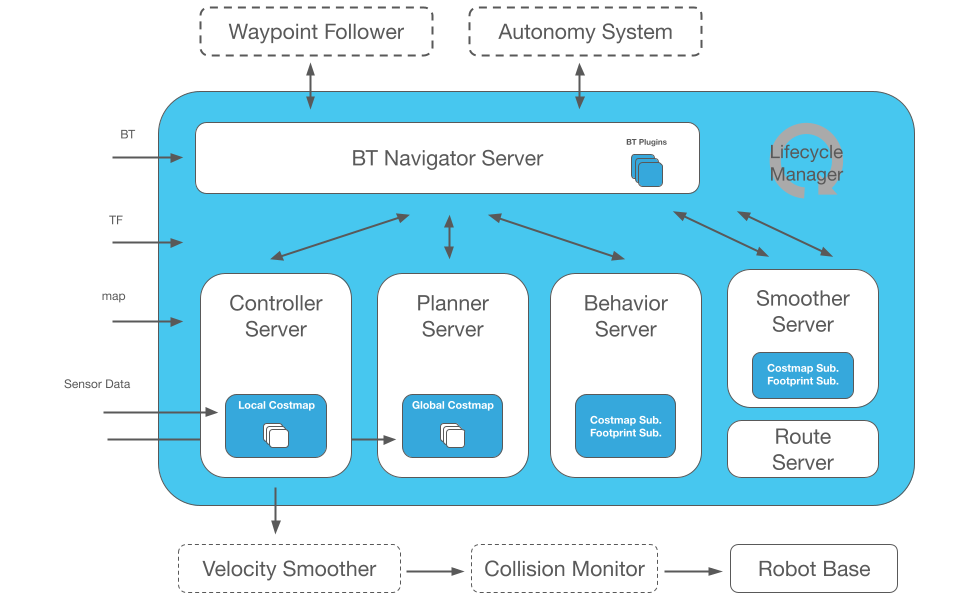
\includegraphics[width=0.8\linewidth]{img/nav2_architecture.png}
\captionof{figure}{Nav2 architecture}
\end{figure}
\newline
These are also some of the updates that have changed from ROS 1 other less notable changes are the use of:
\begin{itemize}
	\item \textbf{Behavior trees}\cite{Colledanchise_2018}: gives to Nav2 a structure for completing a series of tasks in a human readable way. Their structure is similar to a tree and allow to create complex system that can be tested with different tools. The package used for this is BehaviorTree.CPP\footnote{\href{https://www.behaviortree.dev/}{https://www.behaviortree.dev/}} that respect others allow to link different tree.
	\item \textbf{nav2\_util LifecycleNode} is a wrapper of rclcpp\_lifecycle LifecycleNode of the standard structure of ros as described in Nodes \ref{LifecycleNode} and add a bond connection to the lifecycle manager, node that knows the states of each node, and allow to  transition down its lifecycle nodes for safety if some node has crashed.
	\item \textbf{Action Server}: the functionality are described in the structure of ROS \ref{Action} and they are implemented in Nav2 for the interaction with the Behavior Tree (BT) like NavigationToPose (move to a location), NavigationThroughPoses (allow to select multiple waypoints), etc.
\end{itemize}
The control is based on this nodes:
\begin{itemize}
	\item \textbf{controller\_server} is the node that handle the request for moving the robot, using tree plugins progress checker (check if the robot has make some progress in following the path), goal checker (check if the robot has reached the goal position) and controller (generate the velocity command using the \textbf{local costmap} to move the robot avoiding collision)
	\item \textbf{planner\_server} is the node that handle the request for calculate the path, using a loaded plugin planner, to reach a position using the \textbf{global costmap} and the data from sensors.
	\item \textbf{bt\_navigator} is a Behavior Tree-based implementation of navigation that implement the NavigateToPose, NavigateThroughPoses, and other task interfaces to increment the flexibility during navigation.
	\begin{figure}[h]
		\centering
		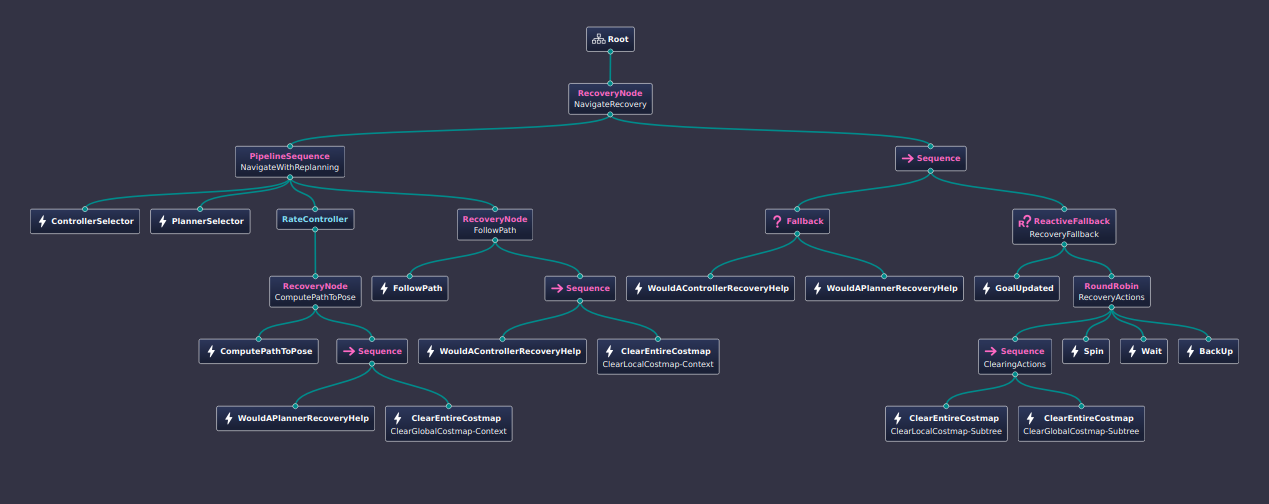
\includegraphics[width=0.8\linewidth]{img/bt2_nav2.png}
		\captionof{figure}{Nav2 bt navigation TOCECK}
	\end{figure}
	\item \textbf{smoother\_server}
	\item \textbf{behavior\_server}
	\item \textbf{waypoint\_follower}
	\item \textbf{velocity\_smoother}
	\item \textbf{global\_costmap}
	\item \textbf{local\_costmap}
\end{itemize}
\section{Cartographer}
\chapter{Review of related work on porting navigation stack from ROS1 to ROS2}
\chapter{Overview of open source fleet management systems, particularly Open-RMF}
\section{Open-RMF description}
...




%\part{Methodology}
In this part we will discuss all the procedure that took place from building our testing platform, based on the Rover Mini and the sensors used. Setting up the Nav2 navigation stack. The procedure used to port the Global planner from ROS 1 to ROS 2. How we integrate the system and the software that is used to setup the Open-RMF system.
\chapter{Description of research platform and hardware used}
The robot is a 4 wheel drive (WD) skid-steering (see Figure \ref{fig:RoverRobotics Rover Mini})that has a maximum speed of 12.87 km/h with a payload of 45,36 kg. With an operating time of Operating Time 60-90 minutes active or max 6 hours in idle. The company offer the code to control it and also to simulate on Gazebo on github\footnote{\href{https://github.com/RoverRobotics/roverrobotics_ros2}{https://github.com/RoverRobotics/roverrobotics\_ros2}}. The code is steel tested only for ROS 2 Humble, this is going to be our version of ROS 2 that we are going to use for navigation on the Rover.\\
For controlling it, the rover give a USB terminal for connecting to a PC or single board computer. For this purpose we are using a Mini PC where there is all the control of all the navigation based on Nav2.
The Mini PC is a Beelink SER3-E-16512EJ0W64PRO with a Ryzen 7 3750H Picasso processor which is a quad-core 8-thread 2.3 GHz mobile processor boosting to 4.0 GHz with Radeon RX Vega 10 Graphics.
The power that it's necessary from it to work will be took from the Rover that can provide 19V.
\begin{figure}[h]
	\centering
	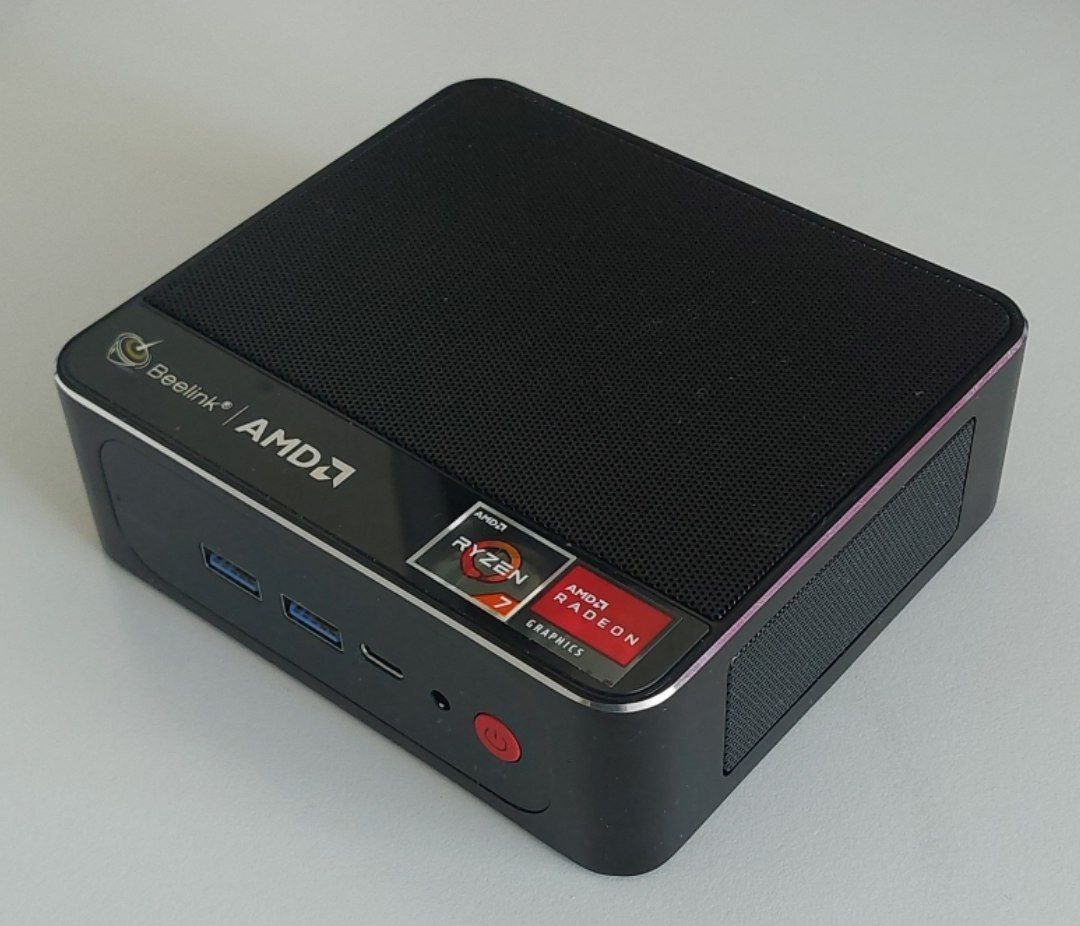
\includegraphics[width=0.4\linewidth]{img/miniPC.jpg}
	\captionof{figure}{Mini PC used}
\end{figure}\\
On top of that to increase the estimation of odometry we will mount an IMU Witmotion (WIT) JY901B. A 9-Axis Combined IMU/Magnetometer/Altimeter (linear accelerations, angular velocities, Euler angles, magnetic field, barometry, altitude). The data from the sensor use a TTL/UART protocol that are collected using the libeary Witmotion Sensors UART Connection Library\cite{andrei_vukolov_2022_7017118},using a channel bridge chip USB to serial, and then published into ROS 2 ecosystem through a node \texttt{witmotion\_ros} using the code from this repo in github ElettraSciComp/witmotion\_IMU\_ros\footnote{\href{https://github.com/ElettraSciComp/witmotion_IMU_ros/tree/ros2}{https://github.com/ElettraSciComp/witmotion\_IMU\_ros/tree/ros2}}.
\begin{figure}[h]
	\centering
	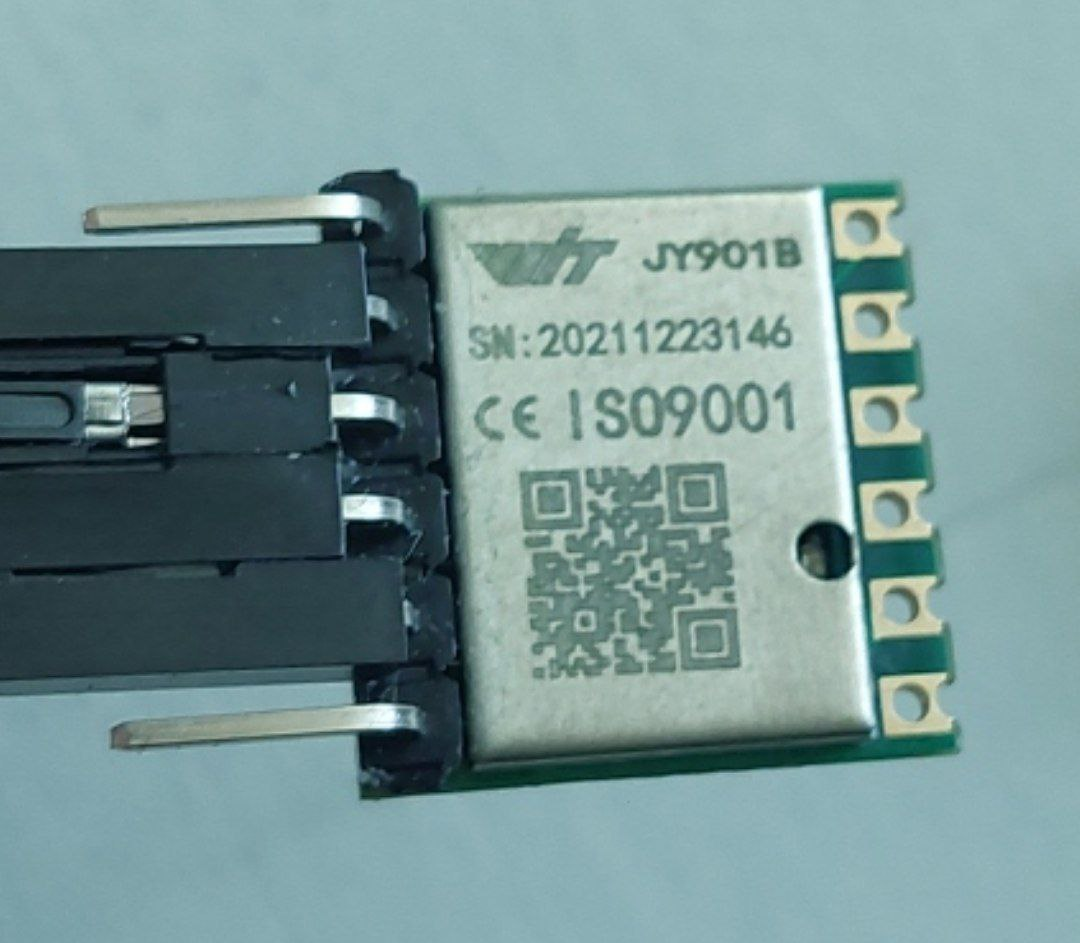
\includegraphics[width=0.4\linewidth]{img/IMU.jpg}
	\captionof{figure}{IMU used}
\end{figure}\\
The last sensor necessary to complete the navigation that is used in localization as described in \ref{ref_map_to_odom} to generate a link between the TF frame \texttt{map} and \texttt{odom} that compensate the errors generated by the model before and see obstacles is a Laser 2D scan because gives as information in all the directions using only a sensor and we built have built only a 2D map, respect at other tools are available \cite{10056144}\cite{vslamComparison2021} that may require more computer power.
The Laser scan used is RPLIDAR S1, 360 degree 2D laser scanner
(LIDAR that is light detection and ranging) with a distance range of 40m on white object and 10m on black ones, a sample rate of 9.2kHz, scan rate from 8 to 15 Hz, so an angular resolution of 0.313-0.587°, accuracy of $\pm$5cm and resolution of 3cm.
The code is available on github Slamtec/sllidar\_ros2 \footnote{\href{https://github.com/Slamtec/sllidar_ros2}{https://github.com/Slamtec/sllidar\_ros2}}.
\begin{figure}[h]
	\centering
	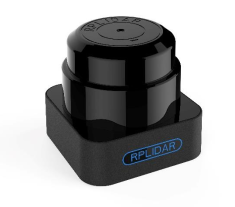
\includegraphics[width=0.4\linewidth]{img/laserScanRPLIDAR.png}
	\captionof{figure}{LIDAR used}
\end{figure}\\
Then all is mounted on the Rover as in the following picture. The couse for this topology is that:
\begin{figure}[h]
	\centering
	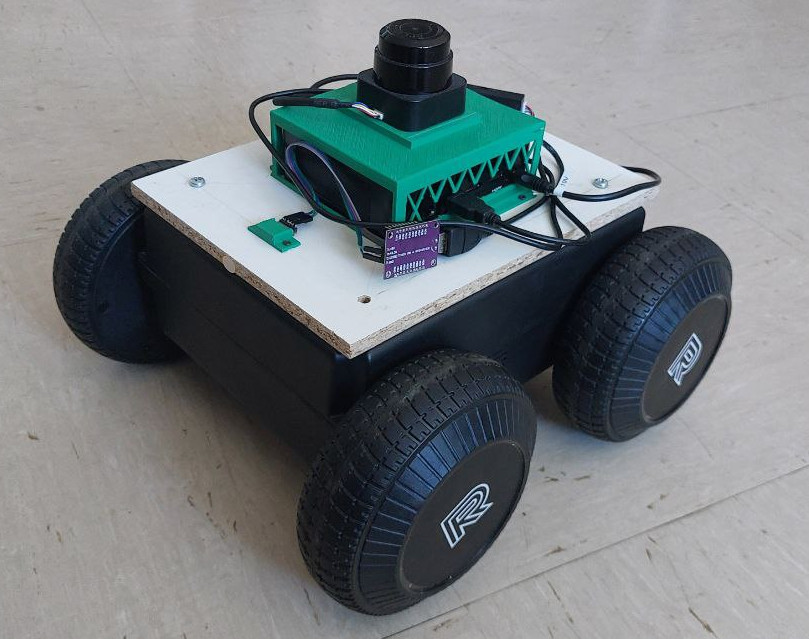
\includegraphics[width=0.4\linewidth]{img/RoverwithSensor.jpg}
	\captionof{figure}{LIDAR used}
\end{figure}\\
\chapter{Steps taken to port the navigation stack from ROS 1 to ROS 2}
\chapter{Hardware adaptation process from Rover Zero to Rover Mini}
\chapter{Integration of the navigation stack with Open-RMF}
\chapter{Testing and evaluation of the system}



%
\part{Results and Analysis}

\chapter{Presentation of results from testing and evaluation}
This part is divided based on the differents thing that have been completed:
\begin{itemize}
	\item porting the planner DStarGlobalPlanner from ROS 1 to ROS 2.
	\item given the robot platform rover mini build an autonomous mobile robot (AMR).
	\item given an the AMR jobot based on ROS 1 port it to ROS 2.
	\item implement the Open-RMF middleware using these robots.
\end{itemize}
\section{Porting the planner}
We have successfully port the code to ROS 2 and used for navigation. These are some output plan generated by the planner with different configuration parameters. More info about of the funtionality of the pramaters are described in its paper.
\\
\begin{figure}[h]
	\centering
	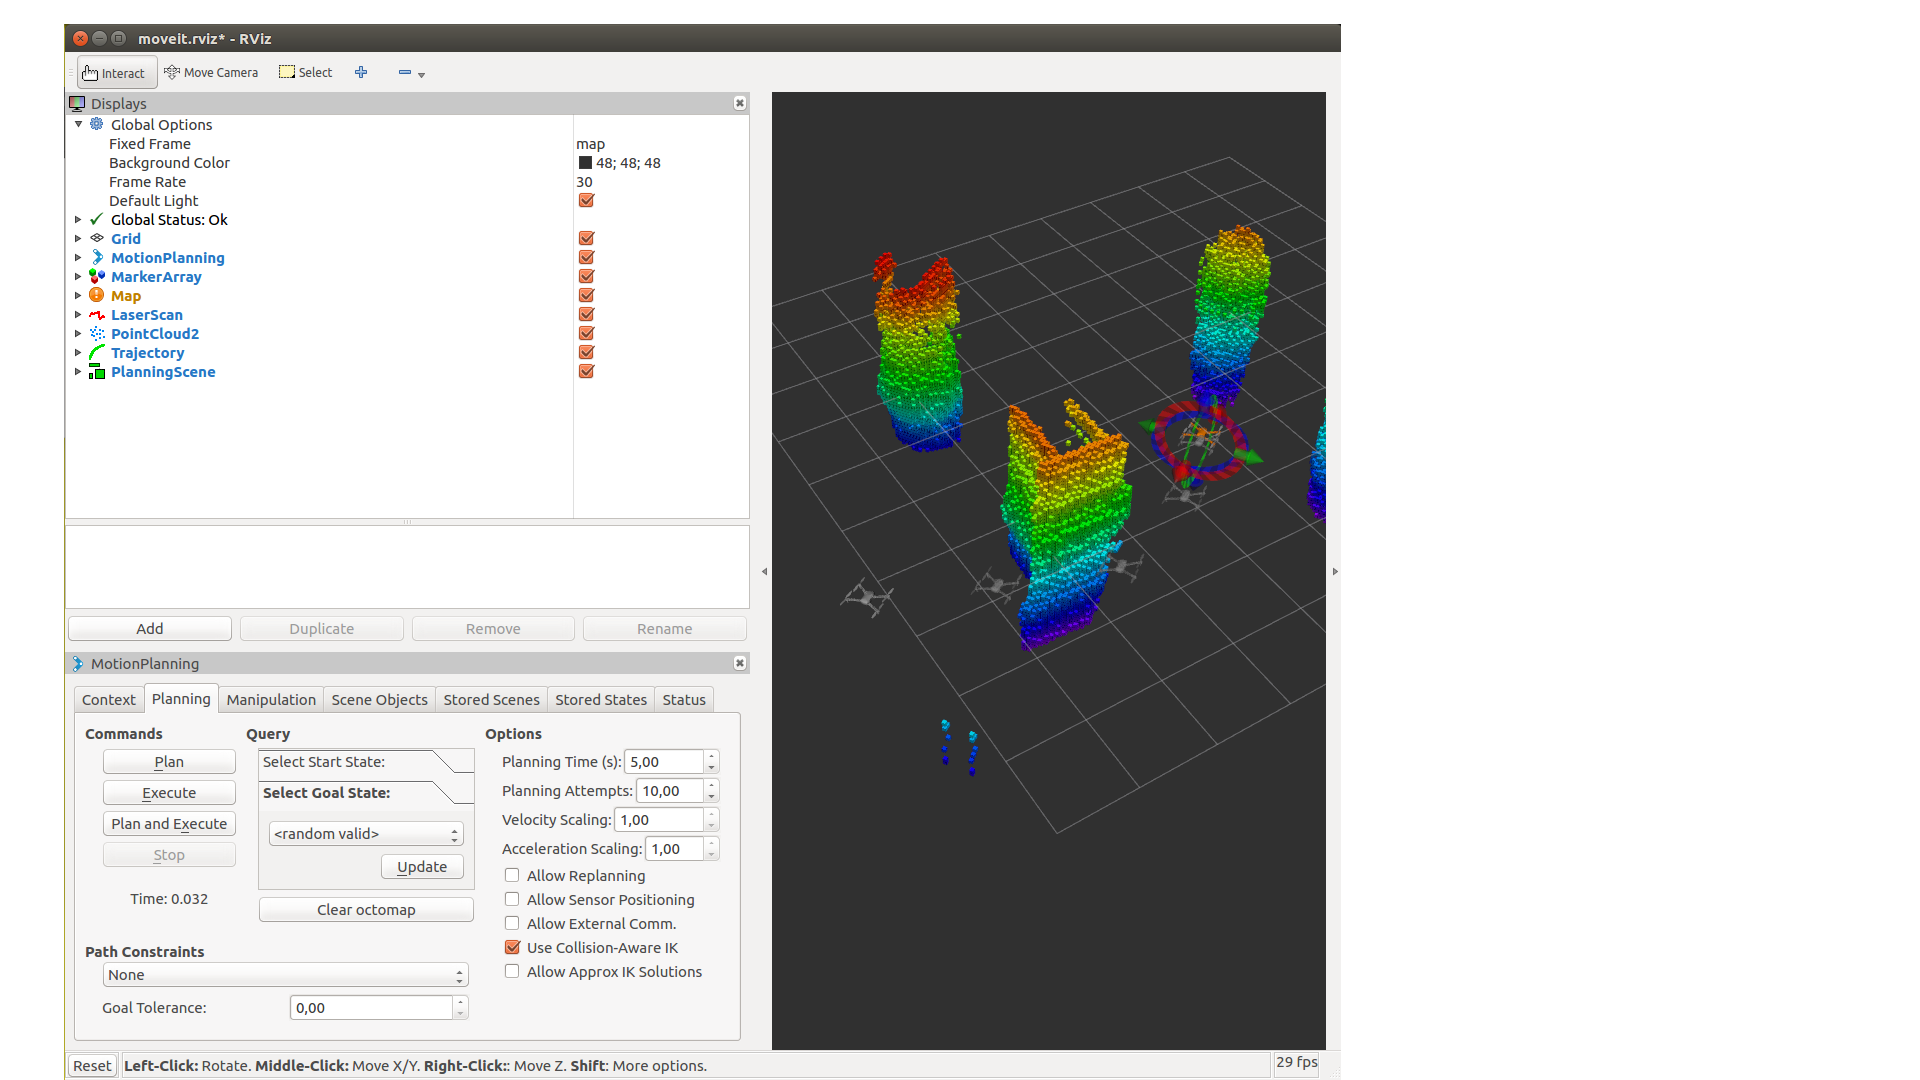
\includegraphics[width=0.7\linewidth]{img/rviz.png}
	\captionof{figure}{results obtained by the planner}
\end{figure}
\\
In the end, the logic transformation between the move\_base logic from ROS 1 to the Planner Server used in ROS 2 for the global planner are based on the implementation of the state machine Lyfecycle and the application of more advanced functionality of the languages used for programming.
\section{RoverRobotics Mini navigation result}
This are some images that display the Mini during navigation:\\
\begin{figure}[h]
\centering
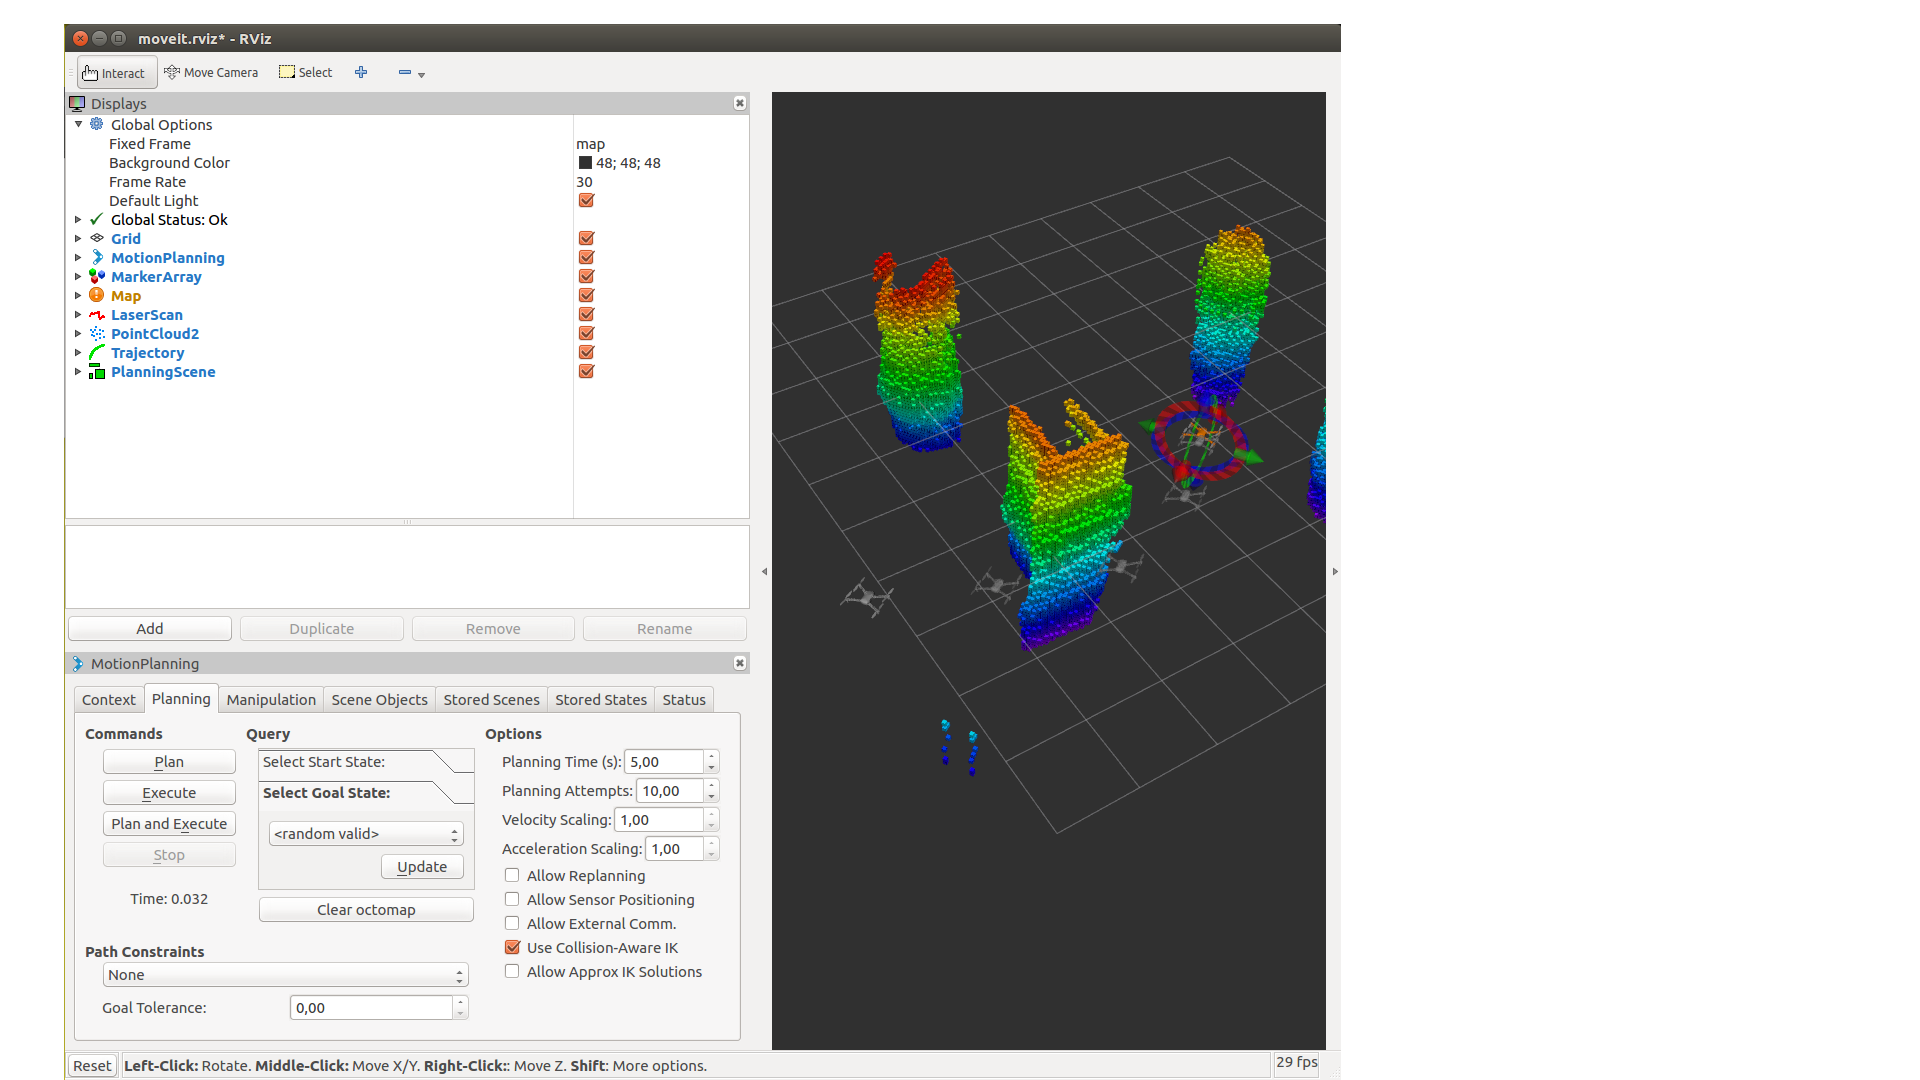
\includegraphics[width=0.7\linewidth]{img/rviz.png}
\captionof{figure}{results navigation of Mini}
\end{figure}
\\
The implementation was enough stray forward, building the robot and then apply the corrected nodes allow as to build a AMR. The tuning of the localization node and the localization node takes some time but is was reduced with the use of rosbag. 
\section{Jobot navigation result}
This are some images that display the Jobot during navigation:\\
\begin{figure}[h]
\centering
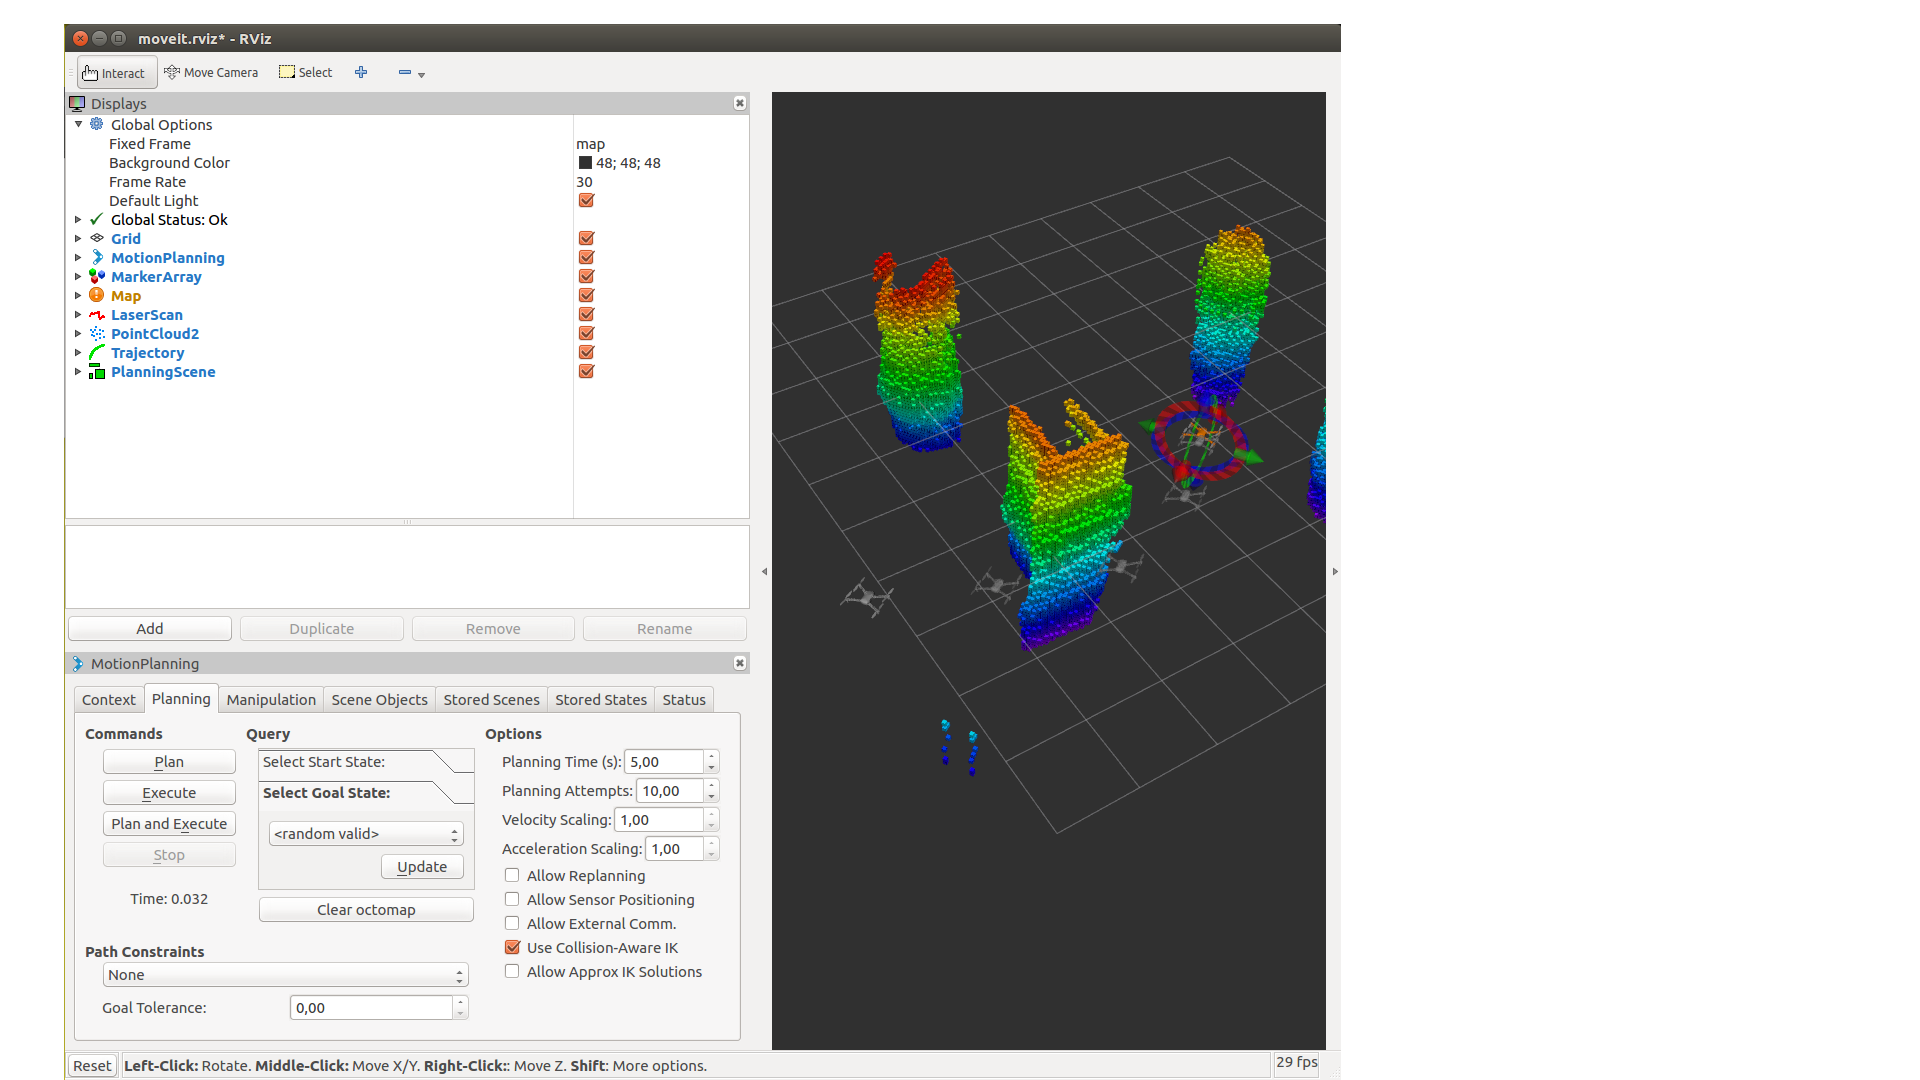
\includegraphics[width=0.7\linewidth]{img/rviz.png}
\captionof{figure}{results navigation of jobot}
\end{figure}
\\
Similar to the Mini, just more tuning.
\section{Open-RMF navigation result}
These are some images of the navigation of the 2 robots\\
\begin{figure}[h]
\centering
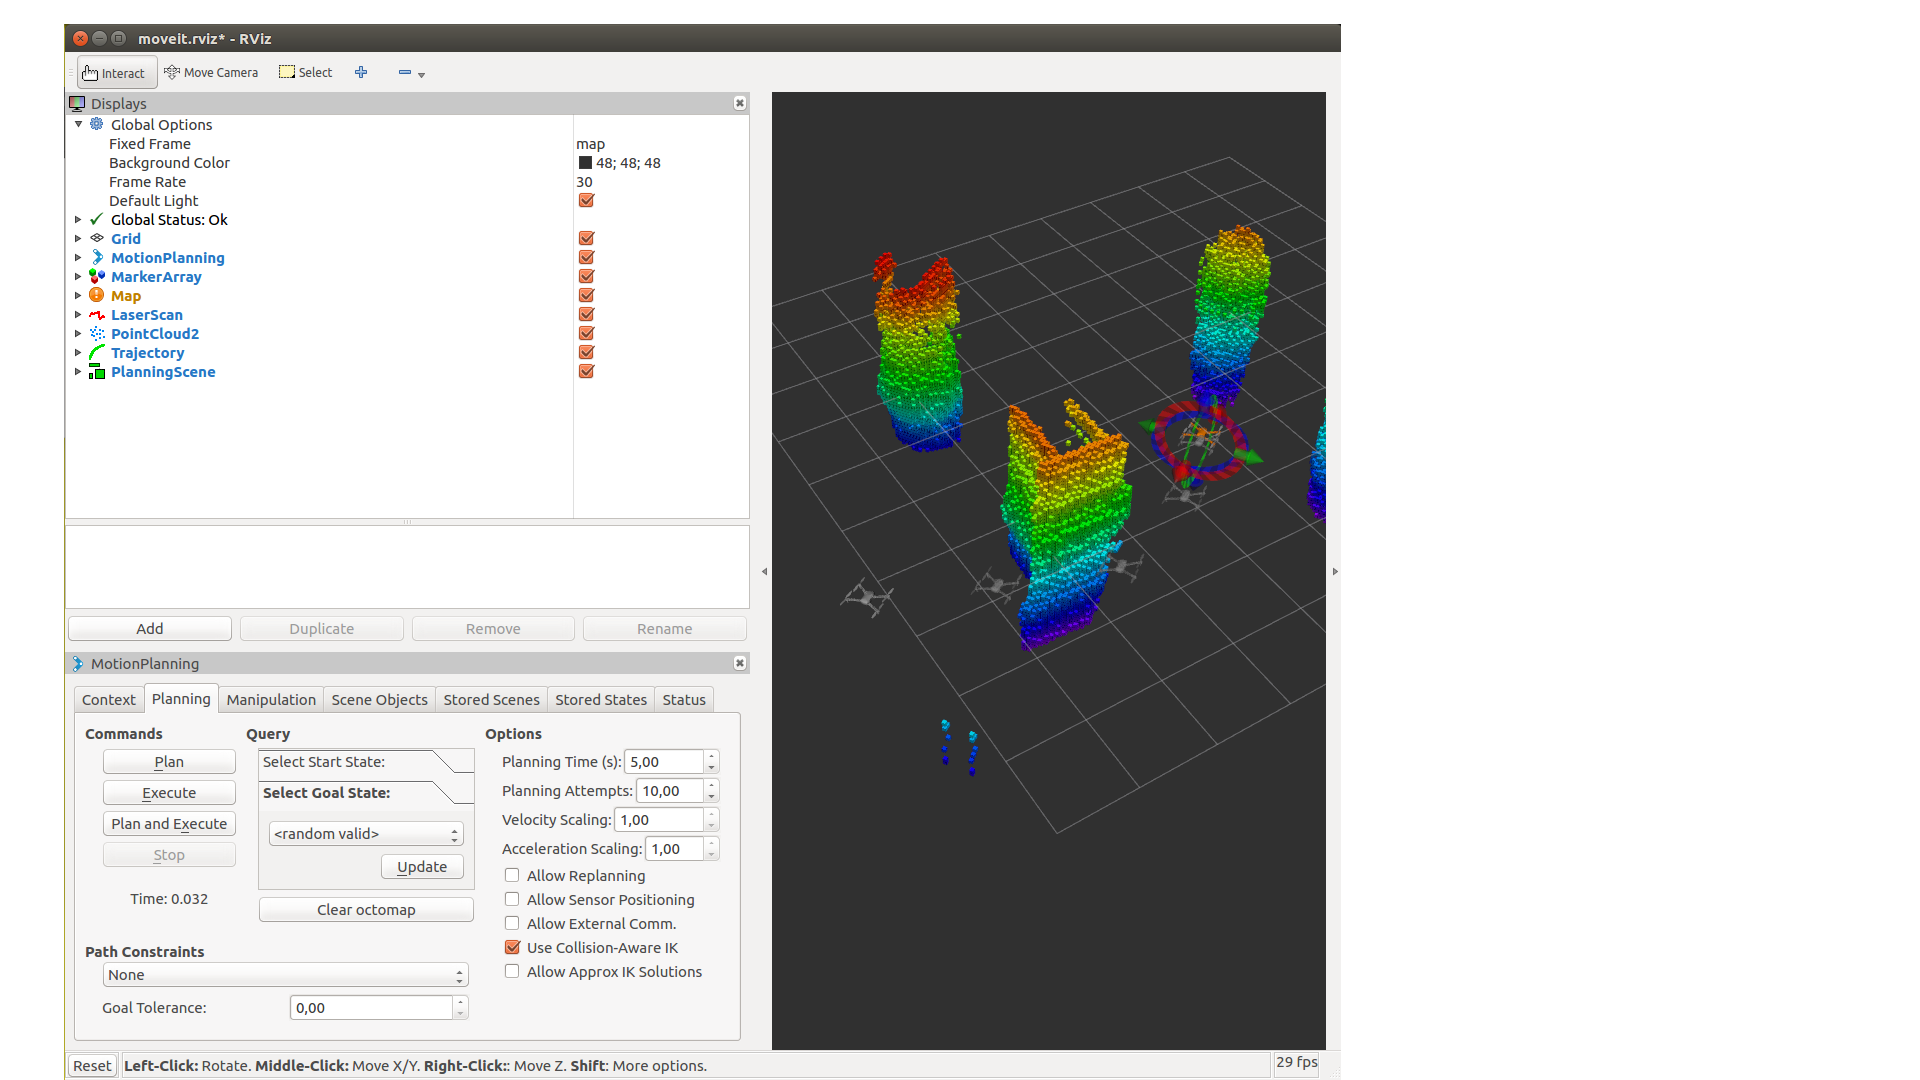
\includegraphics[width=0.7\linewidth]{img/rviz.png}
\captionof{figure}{images navigation of the 2 robots with open-rmf}
\end{figure}\\

\chapter{Comparison of system performance before and after the porting process}
This part is divided in section, in each section we evaluates the following:
\begin{itemize}
	\item calculation time for the planner on Mini rover
	\item navigation response from ROS 1 to ROS 2
\end{itemize}

\section{Planner calculation time comparisation before and after and vs new nav2 planner}
In this section, we present the time required for the global planner node to respond to a request for a path, comparing the performance between the Jobot robot with ROS 1 built-in and the Docker ROS 2 image using the standard planner. \\
\begin{table}[h]
	\centering
	\begin{tabular}{|c|c|c|c|}
		\hline
		Start->End & ROS 1 D-start & ROS 2 D-start & ROS 2 Nav2 \\
		\hline
		ufficio -> magazzino & 1.25 & 1.35 & 1.27 \\
		\hline
		ufficio -> pausa lontana 1 & 1.25 & 1.35 & 1.27 \\
		\hline
		magazzino -> pausa lontana 2 & 1.25 & 1.35 & 1.27 \\
		\hline
	\end{tabular}
	\caption{result planner asking the node}
\end{table}\\
this is some result on rviz\\
\begin{figure}[h]
\centering
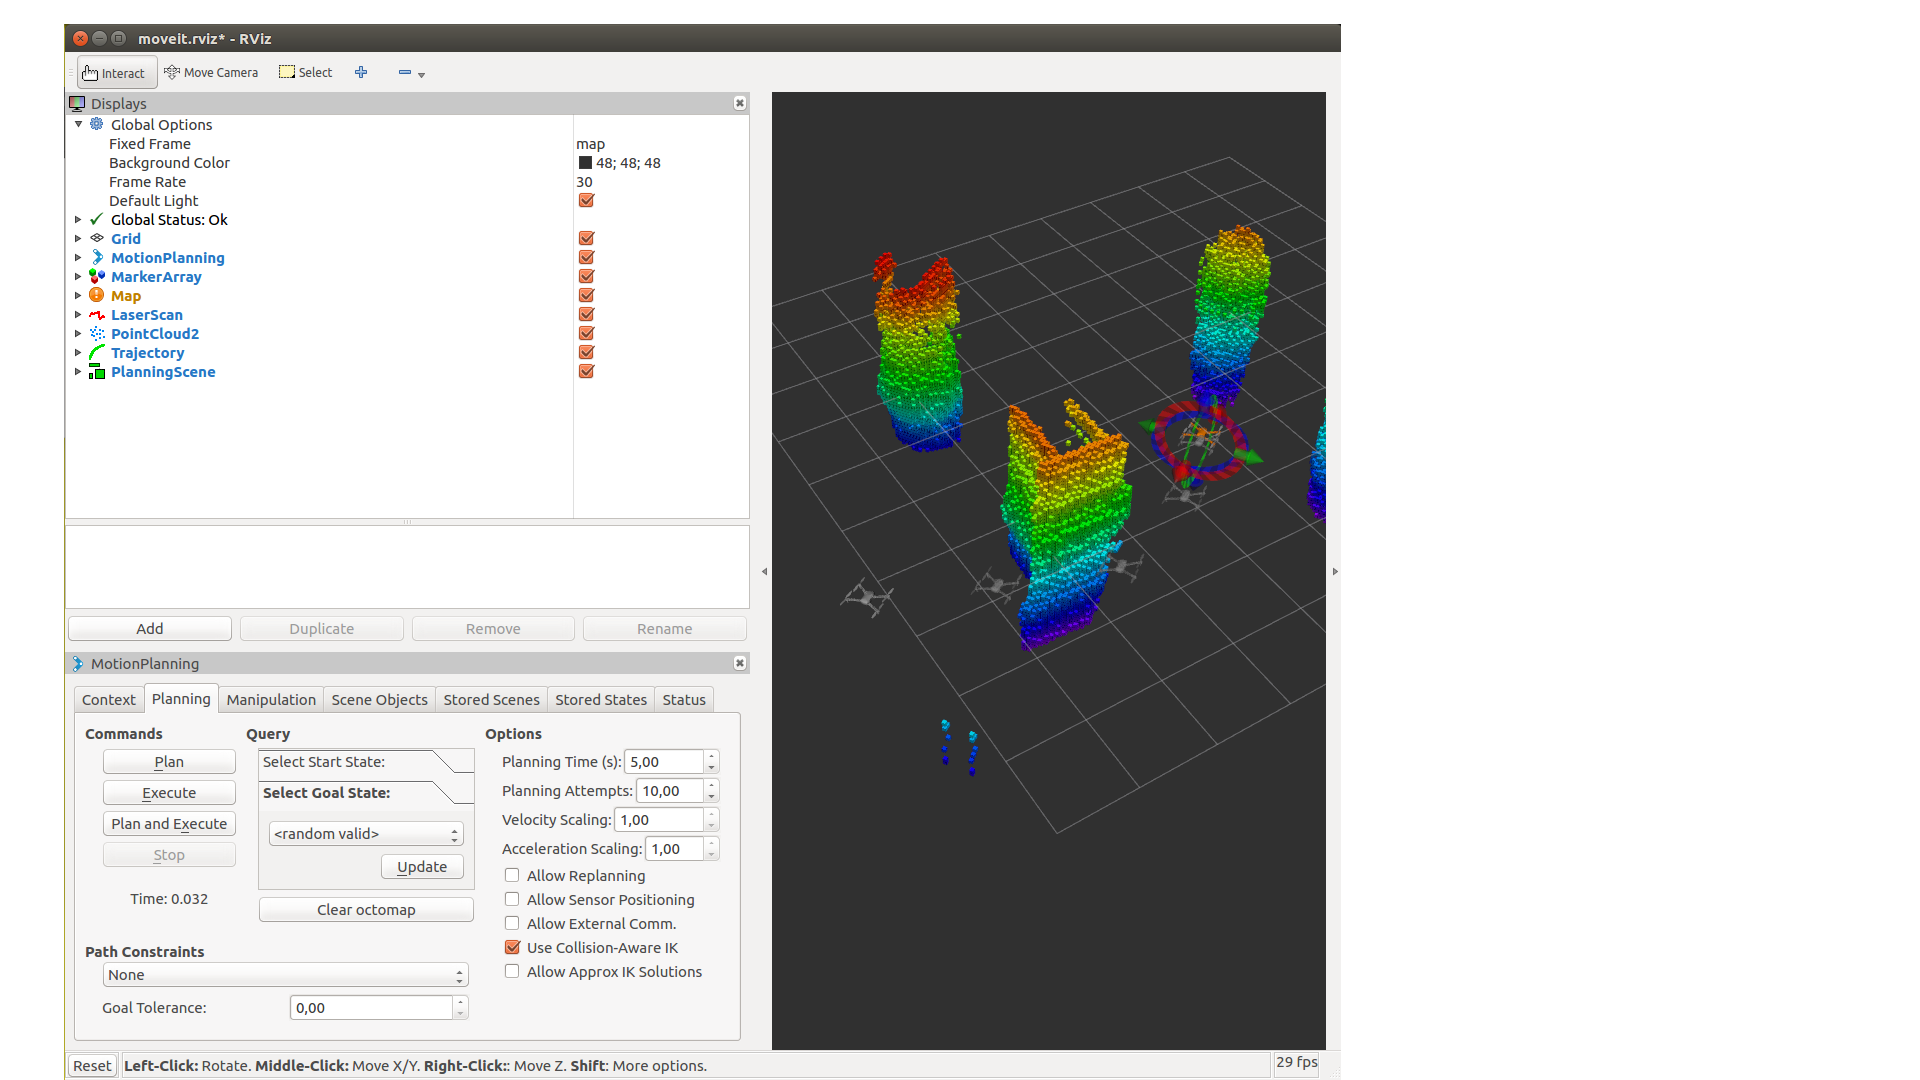
\includegraphics[width=0.7\linewidth]{img/rviz.png}
\captionof{figure}{rviz plan results}
\end{figure}\\
we obtain the following conclusion\\

\section{comparisation jobot navigation}
the test are performed using the same points as used before
\begin{table}[h]
	\centering
	\begin{tabular}{|c|c|c|}
		\hline
		Start->End & ROS 1 D-start & ROS 2 D-start \\
		\hline
		ufficio -> magazzino & 1.25 & 1.35\\
		\hline
		ufficio -> pausa lontana 1 & 1.25 & 1.35\\
		\hline
		magazzino -> pausa lontana 2 & 1.25 & 1.35\\
		\hline
	\end{tabular}
	\caption{result planner asking the node}
\end{table}
we obtain the following conclusion
\chapter{Discussion on the challenges encountered and how they were addressed}
the chalenges are:
\begin{itemize}
	\item high error on localization moving forward, it over estimate the movement comparing the map
\end{itemize}




%\part{Conclusion and Future Work}
%\part{Appendices}
\chapter{Simulation}
In this part i will write some useful information for running the simulation.
All test were done on debian based machine:
To see the graphical interface launched in the docker container you need to have to share the access to the X server using the command \texttt{xhost local:root}.


today the tool for converting the data are 
\href{https://www.ros.org/blog/noetic-eol/}{https://www.ros.org/blog/noetic-eol/}


implement also \href{https://github.com/ros-navigation/navigation2/tree/main/tools/planner\_benchmarking}{planning benchmark}

describe and \textcolor{red}{use} composition in nav2 to obtain better performance \cite{10132508}



Inoltre per gestire il traffico sulla rete utilizzeremo zenoh (Zero Overhead Network Protocol) ed il bridge per ros2 zenoh-bridge-ros2dds che è  pub/sub/query protocol unifying data in motion, data at rest and computations. It elegantly blends traditional pub/sub with geo distributed storage, queries and computations, while retaining a level of time and space efficiency that is well beyond any of the mainstream stacks. data liberator protocol. Zenoh liberates data in several dimensions. 


with chatgpt possiamo gestire il robot in due modi: si ferma ed esegue l'azione non communicando con rmf (la linea rimane bloccata dal suo passaggio) 


%\addcontentsline{toc}{chapter}{Bibliography}
%\bibliography{cap/references.bib}
\printbibliography
\end{document}